%------------------------------------------------------------------------------
% Code
%------------------------------------------------------------------------------

% Command based on: https://tex.stackexchange.com/questions/266811/define-a-new-command-with-parameters-inside-newcommand
\newcommand{\codeName}[1]{\expandafter\newcommand\csname #1\endcsname{\inlineHs{#1}}}

% Used for showing what the blue-highlighted text is, in the reading notes section
\codeName{ExampleText}

% Defines commands to be used in poster and thesis

\newcommand{\swebokScalDef}{This seems to define ``usability
    testing'' with elements of functional and recovery testing}
\newcommand{\swebokElasRef}{only cites a single source
    \textbf{that doesn't contain the words ``elasticity'' or ``elastic''}!}

% for assets/code/example.tex...
\newcommand{\exampleCode}{\begin{codeSnippet}{haskell}{``MultiDefinitions'' (MultiDefn) Definition}{exampleCode}{https://github.com/JacquesCarette/Drasil/blob/051b9881a6417e51e818c6673c5eab0f48bd5af2/code/drasil-theory/lib/Theory/Drasil/MultiDefn.hs\#L45-L56}
-- | 'MultiDefn's are QDefinition factories, used for showing one or more ways
--   we can define a QDefinition.
data MultiDefn e = MultiDefn{
  -- | UID
  _rUid :: UID,
  -- | Underlying quantity it defines.
  _qd :: QuantityDict,
  -- | Explanation of the different ways we can define a quantity.
  _rDesc :: Sentence,
  -- | All possible ways we can define the related quantity.
  _rvs :: NE.NonEmpty (DefiningExpr e)
}
\end{codeSnippet}
}
\newcommand{\refExampleCode}{\Cref{lst:exampleCode}}

% for assets/code/examplePseudocode.tex...
\newcommand{\examplePseudocode}{\begin{pseudocode}{haskell}{Broken QuantityDict Chunk Retriever}{examplePseudocode}
retrieveQD :: UID -> ChunkDB -> Maybe QuantityDict
retrieveQD u cdb = do
    (Chunk expectedQd) <- lookup u cdb
    pure expectedQd
\end{pseudocode}
}
\newcommand{\refExamplePseudocode}{\Cref{lst:examplePseudocode}}

% for assets/code/mainInvalidInputTest.tex...
\newcommand{\mainInvalidInputTest}{\begin{codeSnippet}{python}{Tests for main with an invalid input file}{mainInvalidInputTest}{https://github.com/samm82/Drasil/blob/sysTests/code/stable/projectile/projectile_c_p_nol_b_u_v_d/src/python/test/Control_test.py\#L29-L53}
  # from https://stackoverflow.com/questions/54071312/how-to-pass-command-line-argument-from-pytest-to-code
  ## \brief Tests main with invalid input file
  # \par Types of Testing:
  # Dynamic Black-Box (Behavioural) Testing
  # Boundary Conditions
  # Default, Empty, Blank, Null, Zero, and None
  # Invalid, Wrong, Incorrect, and Garbage Data
  # Logic Flow Testing
  @mark.parametrize("filename", invalid_value_input_files)
  @mark.xfail
  def test_main_invalid(monkeypatch, filename):
      # from https://stackoverflow.com/questions/10840533/most-pythonic-way-to-delete-a-file-which-may-not-exist
      try:
          remove(output_filename)
      except OSError as e: # this would be "except OSError, e:" before Python 2.6
          if e.errno != ENOENT: # no such file or directory
              raise # re-raise exception if a different error occurred


      assert not path.exists(output_filename)


      with monkeypatch.context() as m:
          m.setattr(sys, 'argv', ['Control.py', str(Path("test/test_input") / f"{filename}.txt")])
          Control.main()
      
      assert not path.exists(output_filename)
\end{codeSnippet}
}
\newcommand{\refMainInvalidInputTest}{\Cref{lst:mainInvalidInputTest}}

% for assets/code/projManualViolationReq.tex...
\newcommand{\projManualViolationReq}{\begin{codeSnippet}{haskell}{\acs{projectile}'s manually created requirement for constraint violation behaviour}{projManualViolationReq}{https://github.com/JacquesCarette/Drasil/blob/afb6fb752b8364d2807ced7fc0c1dd6c6aba52b2/code/drasil-example/projectile/lib/Drasil/Projectile/Requirements.hs\#L31-L34}
verifyParamsDesc = foldlSent [S "Check the entered", plural inValue,
    S "to ensure that they do not exceed the" +:+. namedRef (datCon [] []) (plural datumConstraint),
    S "If any of the", plural inValue, S "are out of bounds" `sC`
    S "an", phrase errMsg, S "is displayed" `S.andThe` plural calculation, S "stop"]
\end{codeSnippet}
}
\newcommand{\refProjManualViolationReq}{\Cref{lst:projManualViolationReq}}

% for assets/code/projViolationChoice.tex...
\newcommand{\projViolationChoice}{\begin{codeSnippet}{haskell}{\acs{projectile}'s choice for constraint violation behaviour in code}{projViolationChoice}{https://github.com/JacquesCarette/Drasil/blob/afb6fb752b8364d2807ced7fc0c1dd6c6aba52b2/code/drasil-example/projectile/lib/Drasil/Projectile/Choices.hs\#L120}
    srsConstraints = makeConstraints Warning Warning,
\end{codeSnippet}
}
\newcommand{\refProjViolationChoice}{\Cref{lst:projViolationChoice}}

%------------------------------------------------------------------------------
% Graphs
%------------------------------------------------------------------------------

% Organization of files
\newcommand{\ExampleGraph}{
    \begin{figure*}
        \begin{subfigure}[b]{0.3\linewidth}
            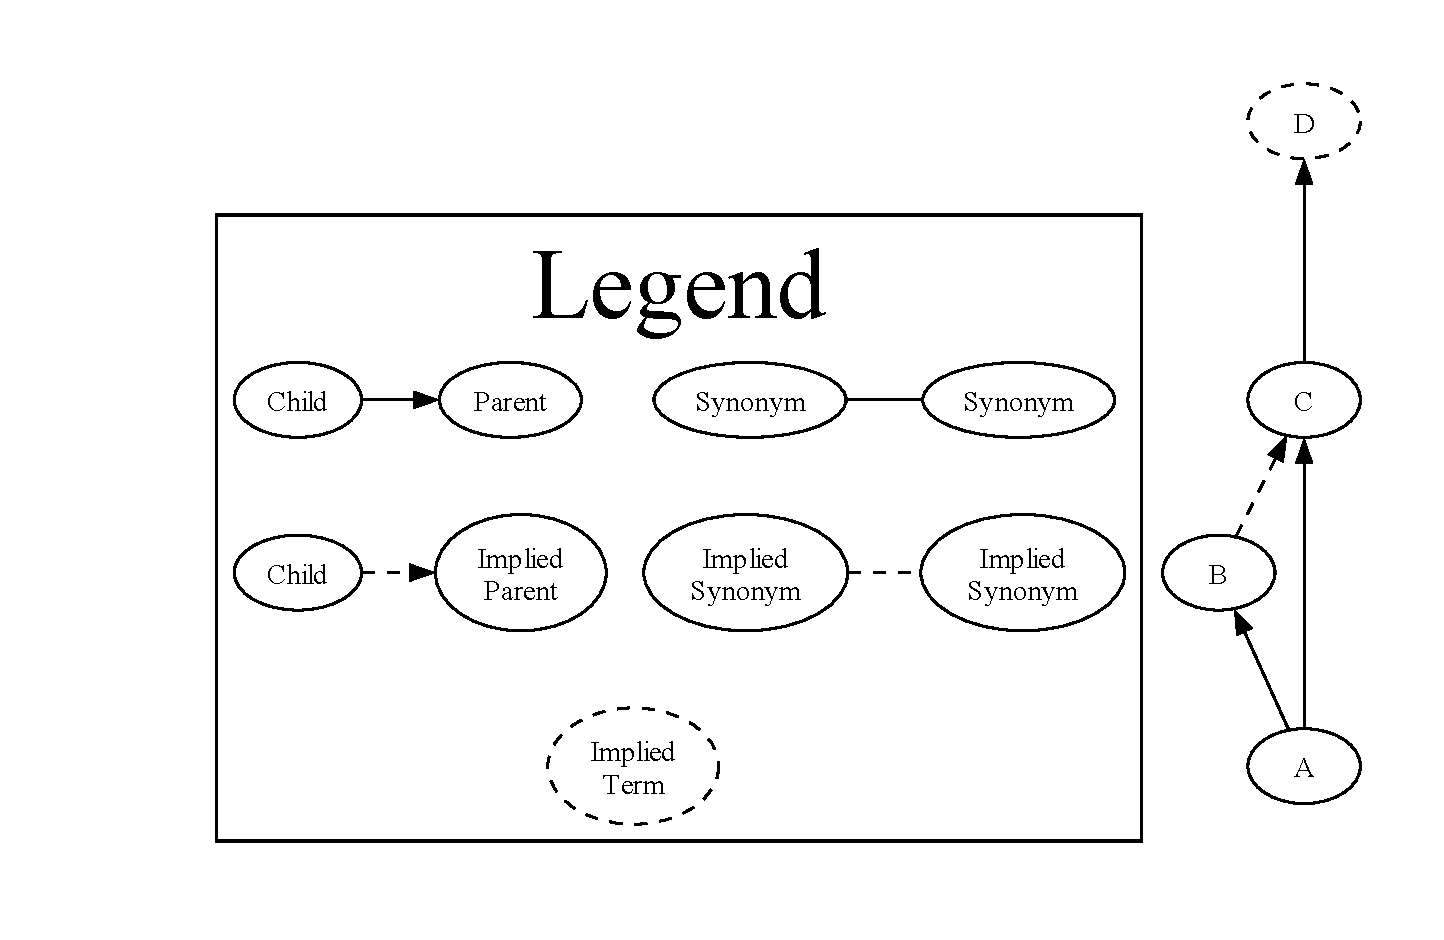
\includegraphics[width=\linewidth]{assets/graphs/ExampleGlossaryGraph.pdf}
            \caption{Graph from \Cref{tab:exampleGlossary}.}
            \label{fig:exampleGraph}
        \end{subfigure}
        \centering
        \begin{subfigure}[b]{0.675\linewidth}
            \centering
            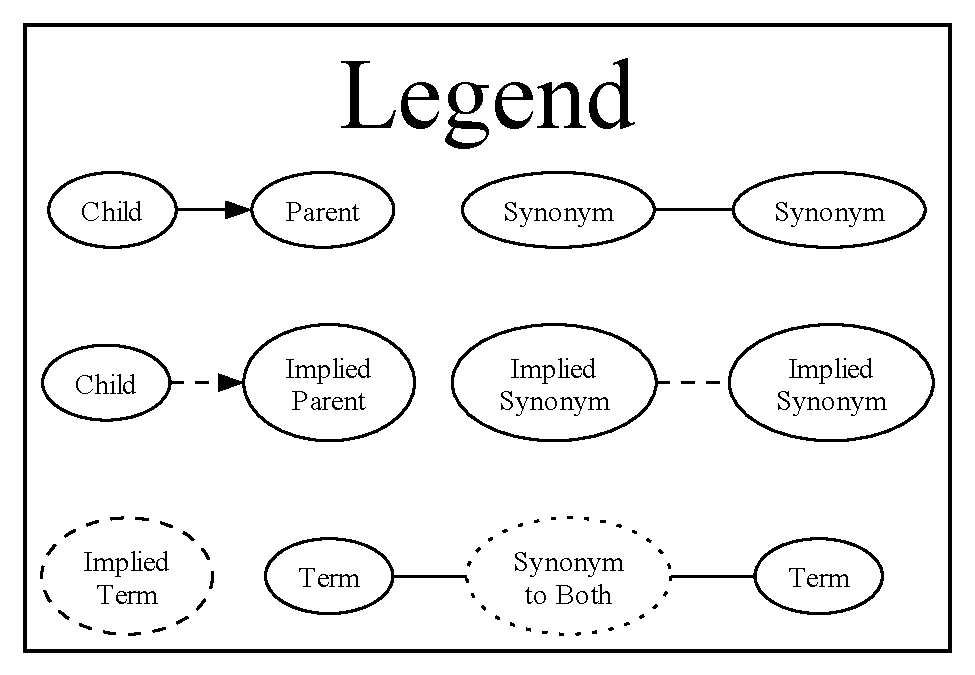
\includegraphics[width=0.8\linewidth]{assets/graphs/manual/manualLegendNonSolidTerms.pdf}
            \hspace{5cm}\begin{subfigure}[t]{0.475\linewidth}
                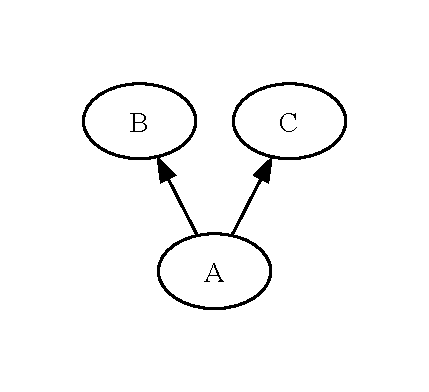
\includegraphics[width=1.1\linewidth]{assets/graphs/rigidExampleGlossaryGraph.pdf}
                \caption{Rigid graph from\\\Cref{tab:exampleGlossary}.}
                \label{fig:rigidExampleGraph}
            \end{subfigure}
            \begin{subfigure}[t]{0.475\linewidth}
                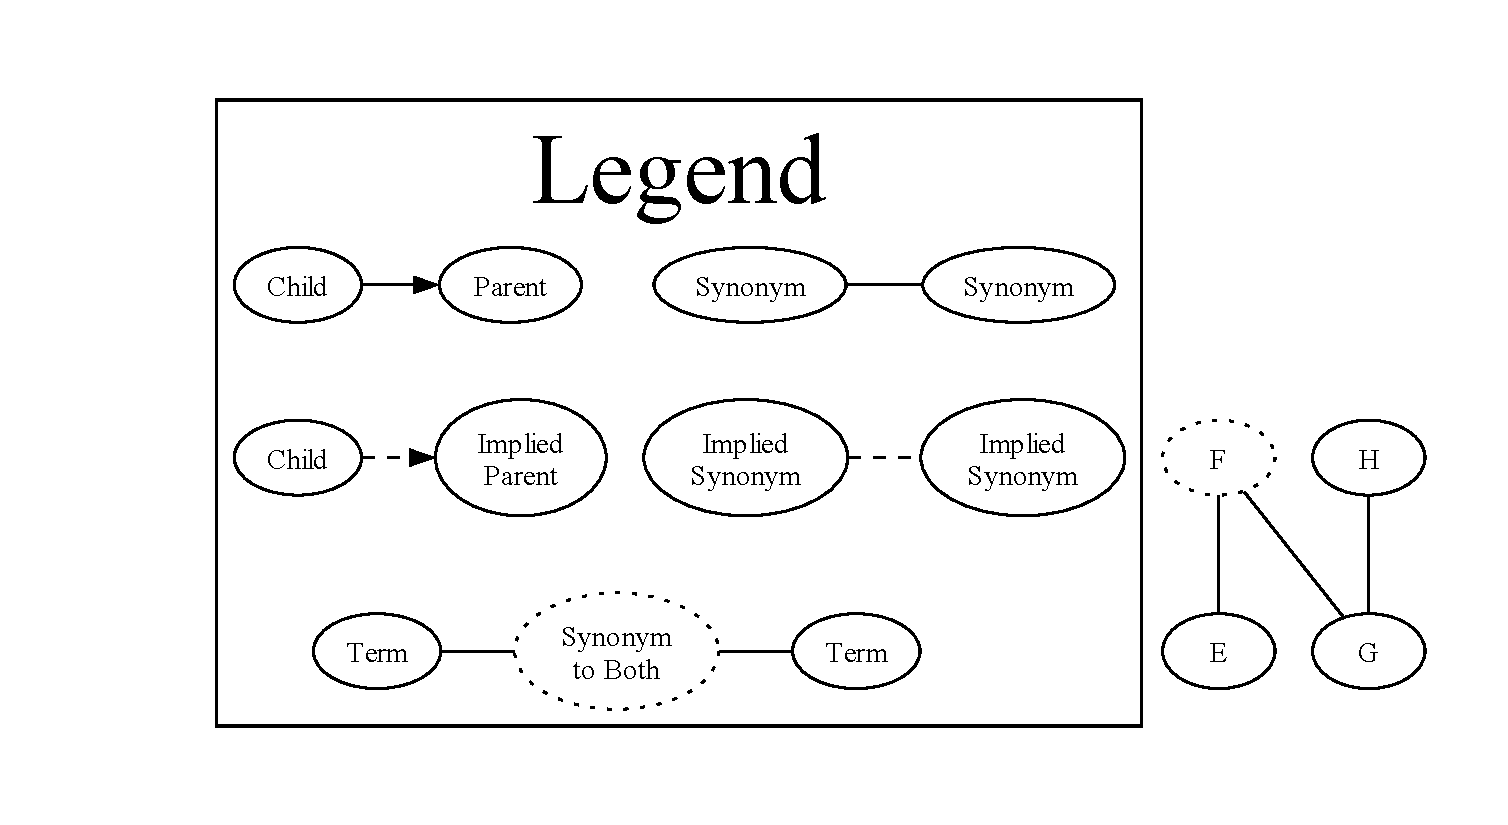
\includegraphics[width=1.1\linewidth]{assets/graphs/SynExampleGlossaryGraph.pdf}
                \caption{Graph from \Cref{tab:synExampleGlossary}.}
                \label{fig:synExampleGraph}
            \end{subfigure}
        \end{subfigure}
        \begin{subfigure}[t]{0.25\linewidth}
            \centering
            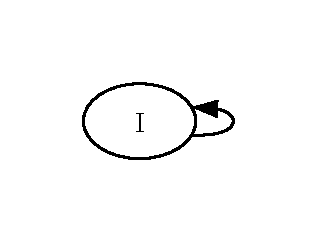
\includegraphics[width=1.2\linewidth]{assets/graphs/SelfExampleGlossaryGraph.pdf}
            \caption{Self-loop graph.}
            \label{fig:selfExampleGraph}
        \end{subfigure}
        \hfill
        \begin{subfigure}[t]{0.425\linewidth}
            \centering
            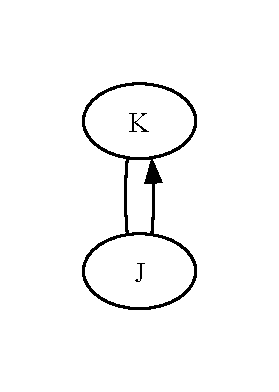
\includegraphics[width=0.6\linewidth]{assets/graphs/ParSynExampleGlossaryGraph.pdf}
            \caption{Graph of a pair of terms with a \hyperref[par-chd-rels]{parent-child} \emph{and} synonym relation.}
            \label{fig:parSynExampleGraph}
        \end{subfigure}
        \hfill
        \begin{subfigure}[t]{0.25\linewidth}
            \centering
            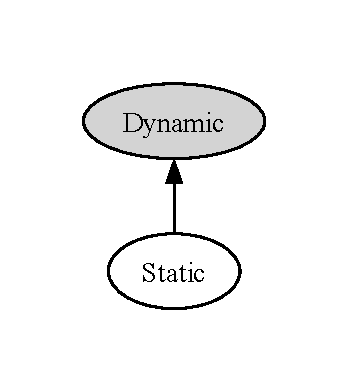
\includegraphics[width=1.4\linewidth]{assets/graphs/StaticExampleGlossaryGraph.pdf}
            \caption{Static graph.}
            \label{fig:staticExampleGraph}
        \end{subfigure}
        \caption{Example generated graphs.}
        \label{fig:exampleGraphs}
    \end{figure*}
}

\newcommand{\recoveryGraphs}{
    % Only top or bottom to comply with IEEE guidelines
    \begin{figure}[bt!]
        \centering
        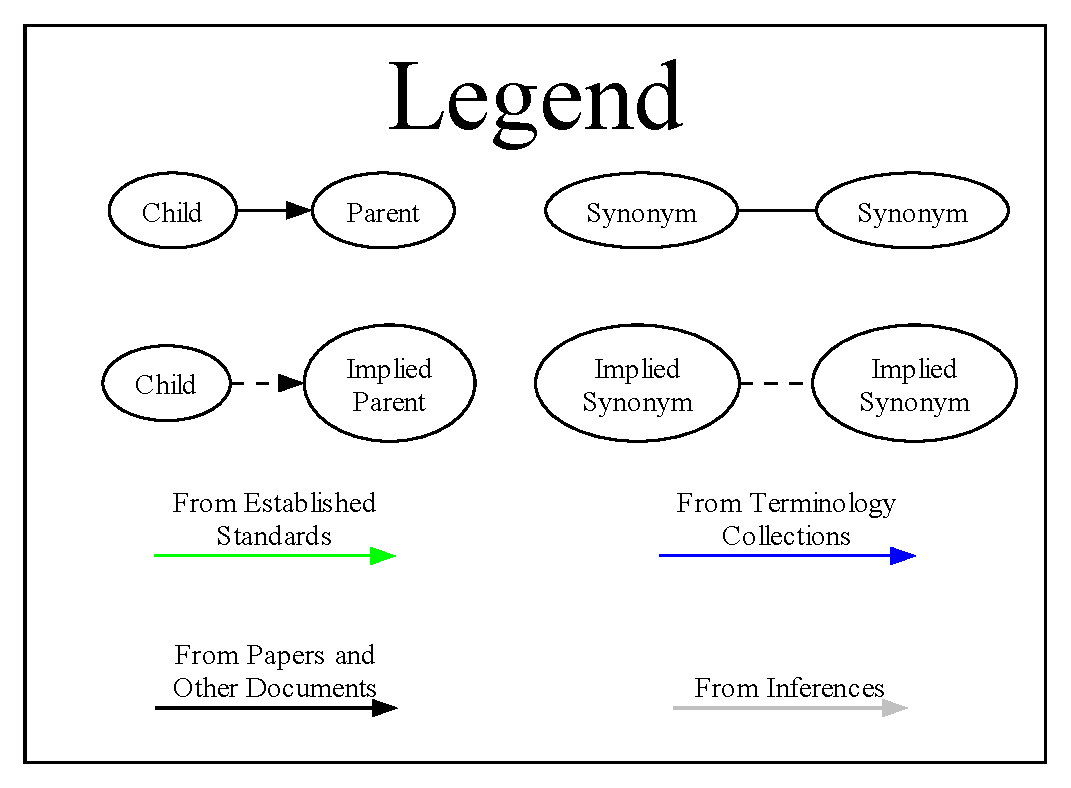
\includegraphics[width=\linewidth]{assets/graphs/recoveryLegend.pdf}
        \begin{subfigure}[b]{.55\linewidth}
            \centering
            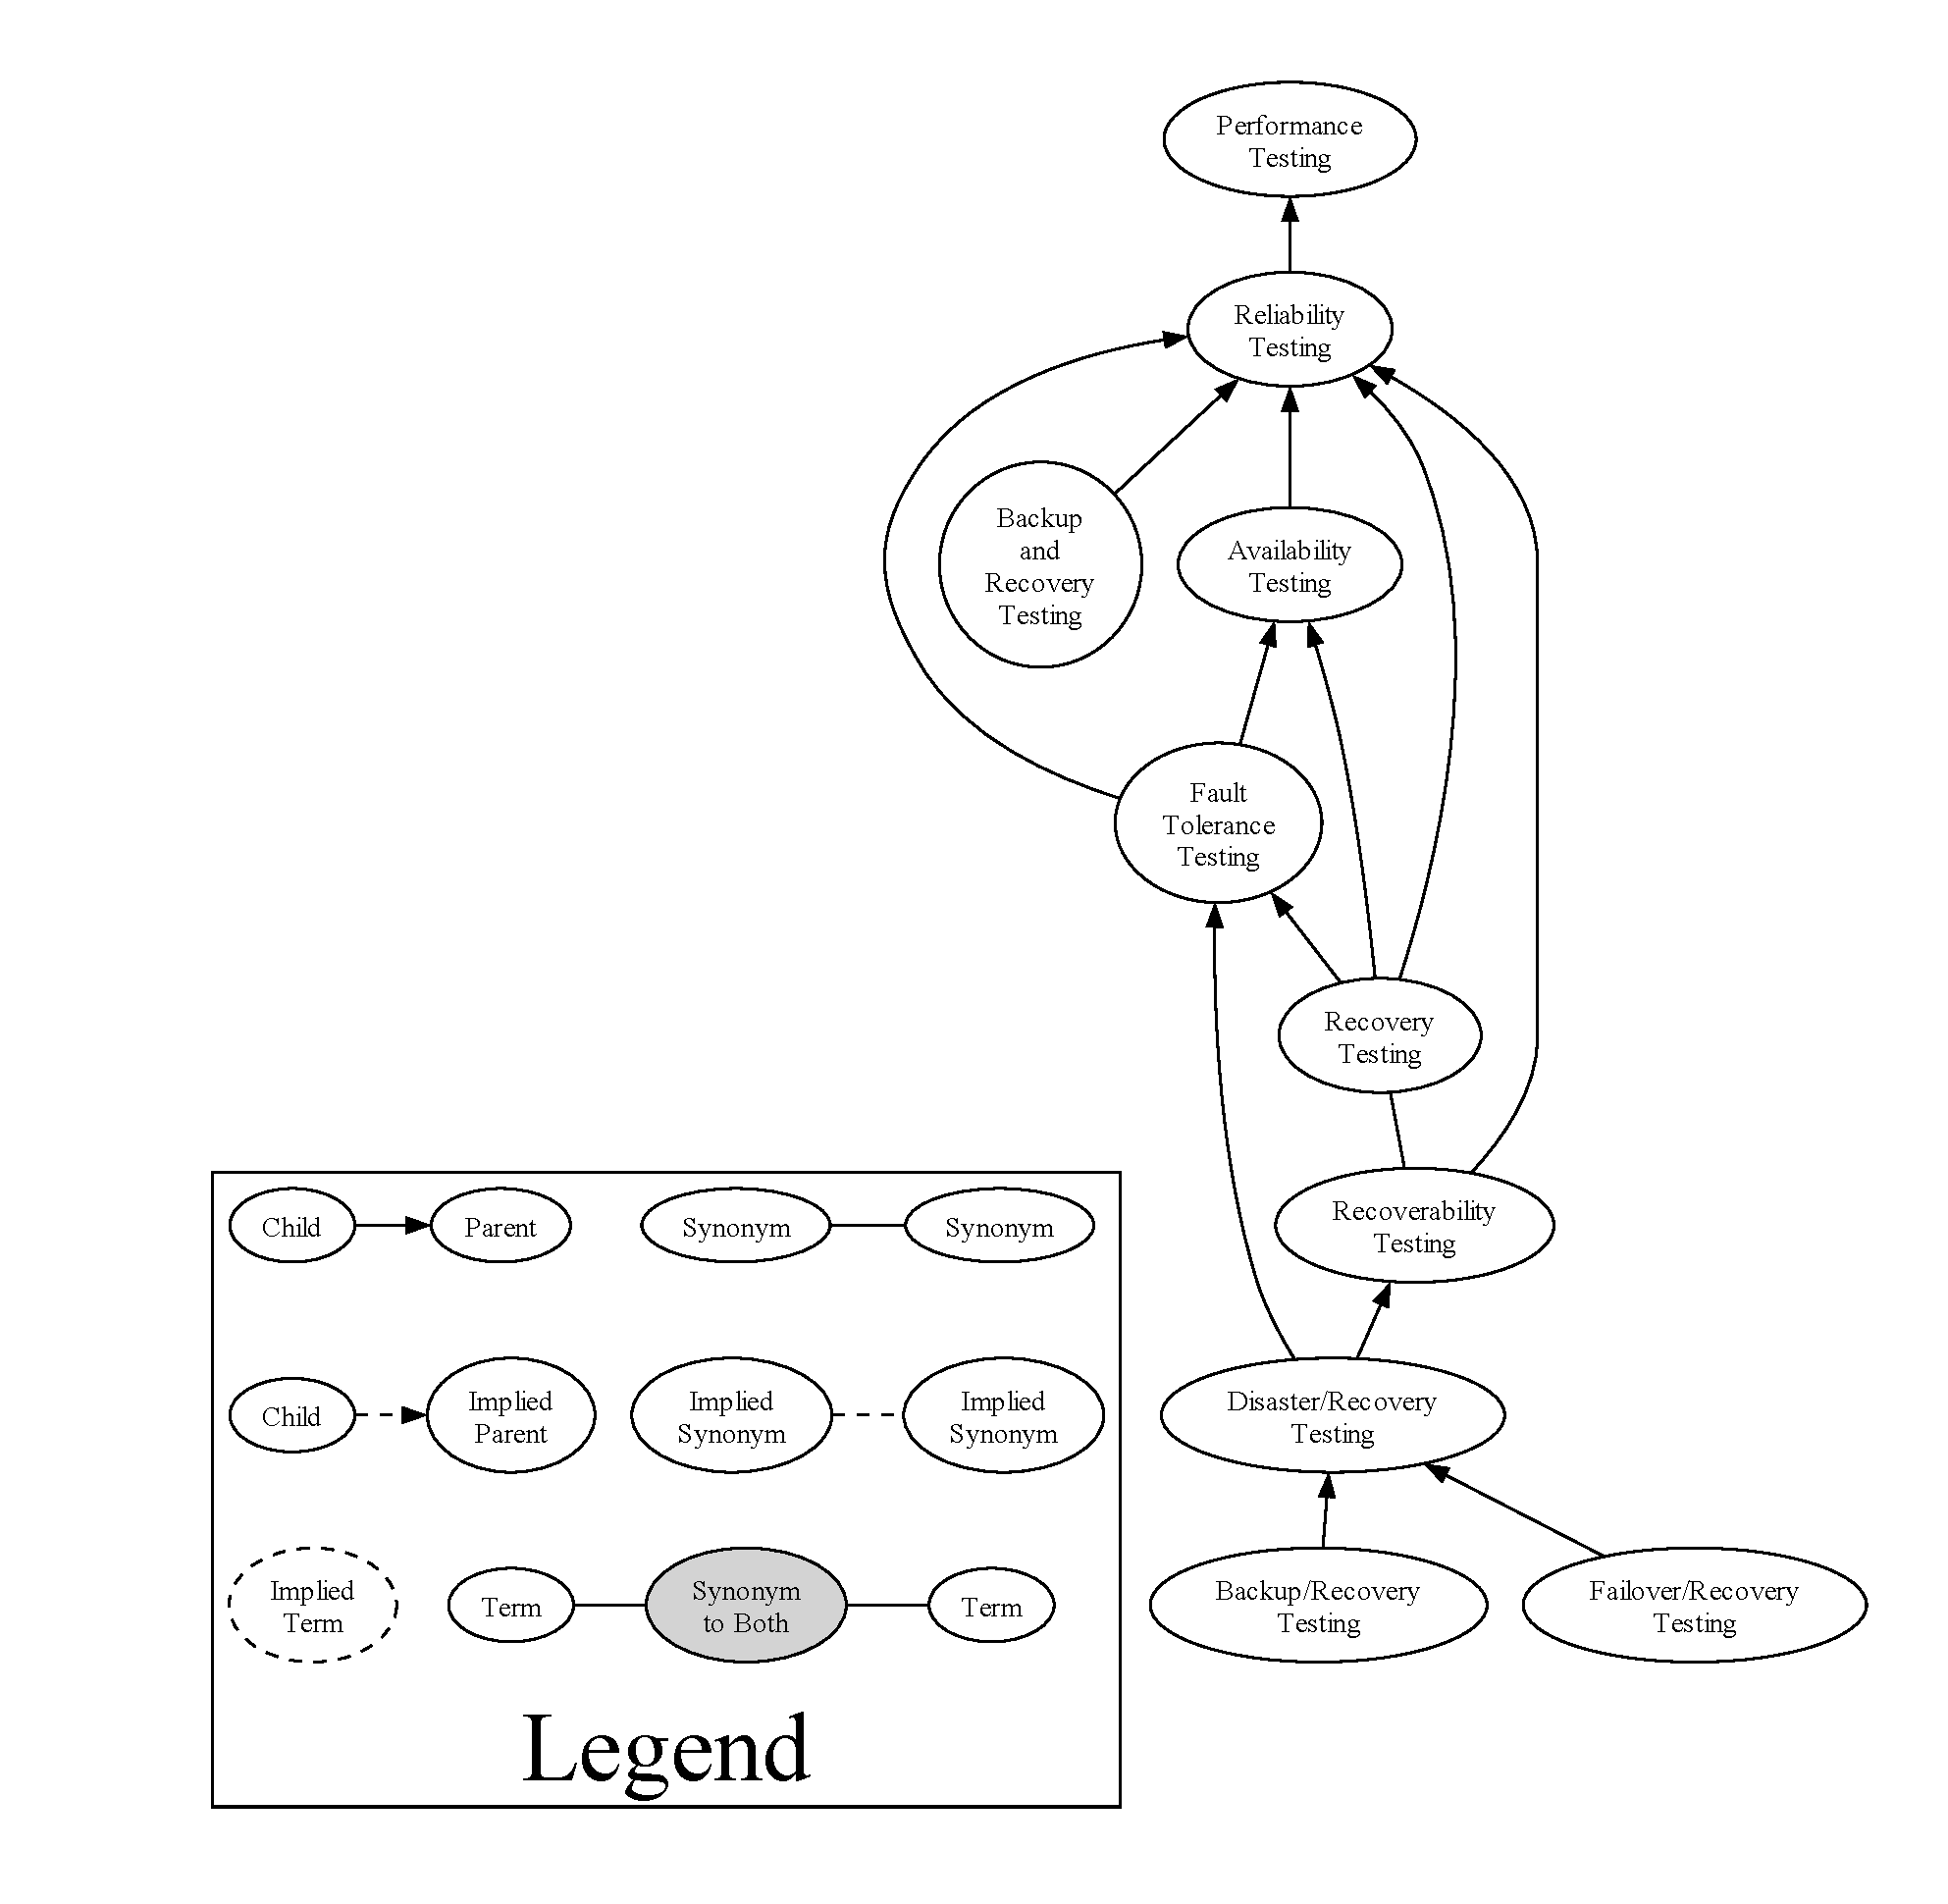
\includegraphics[width=\linewidth]{assets/graphs/recoveryGraph.pdf}
            \caption{Graph of current relations.}
            \label{fig:recovery-graph-current}
        \end{subfigure}
        \begin{subfigure}[b]{.4\linewidth}
            \centering
            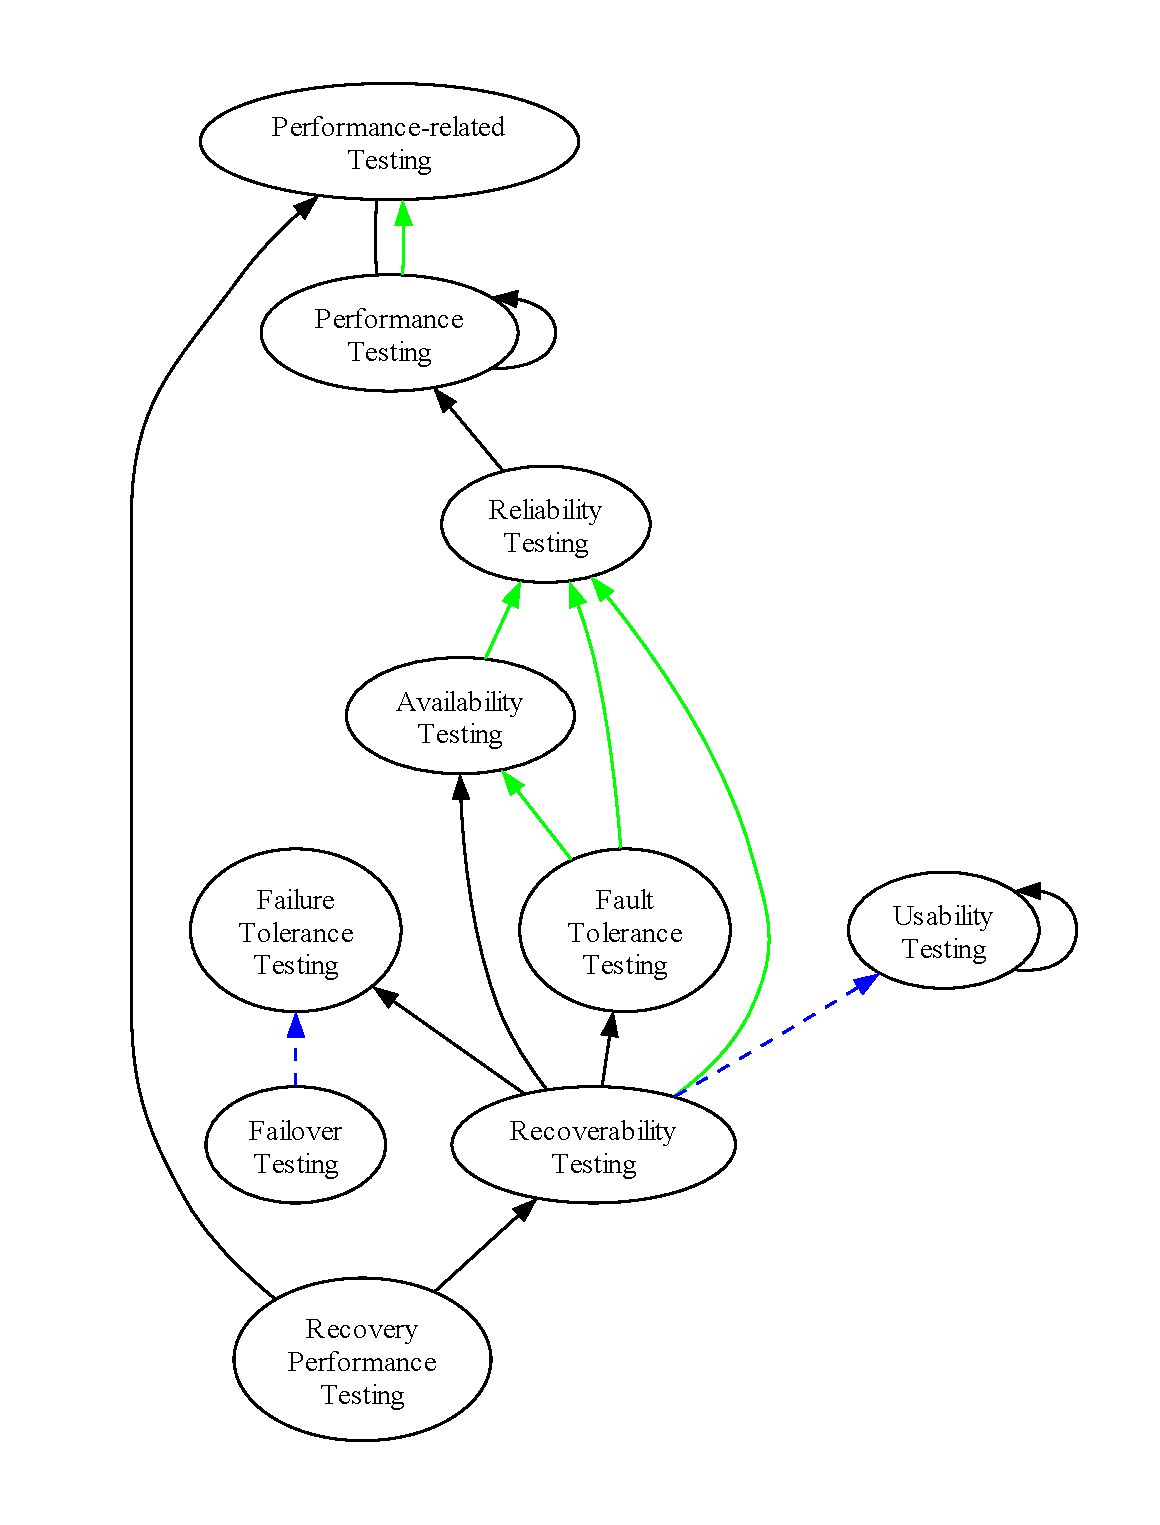
\includegraphics[width=\linewidth]{assets/graphs/recoveryProposedGraph.pdf}
            \caption{Graph of proposed relations.}
            \label{fig:recovery-graph-proposed}
        \end{subfigure}
        \caption{Graphs of relations between terms related to recovery testing.}
        \label{fig:recoveryGraphs}
    \end{figure}
}

\newcommand{\scalGraphs}{
    % Only top or bottom to comply with IEEE guidelines
    \begin{figure}[bt!]
        \centering
        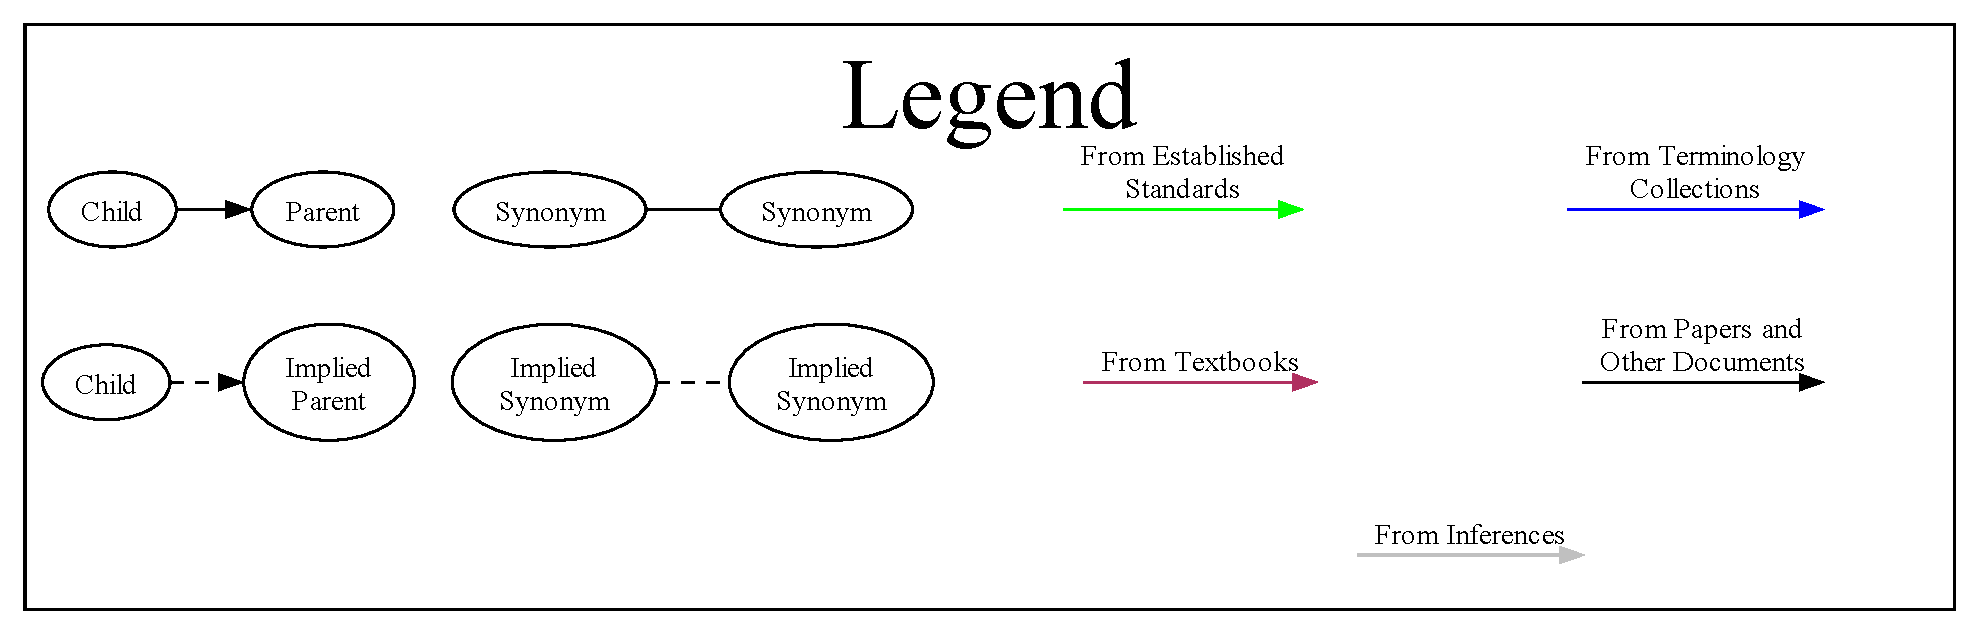
\includegraphics[width=\linewidth]{assets/graphs/scalabilityLegend.pdf}
        \begin{subfigure}[b]{.475\linewidth}
            \centering
            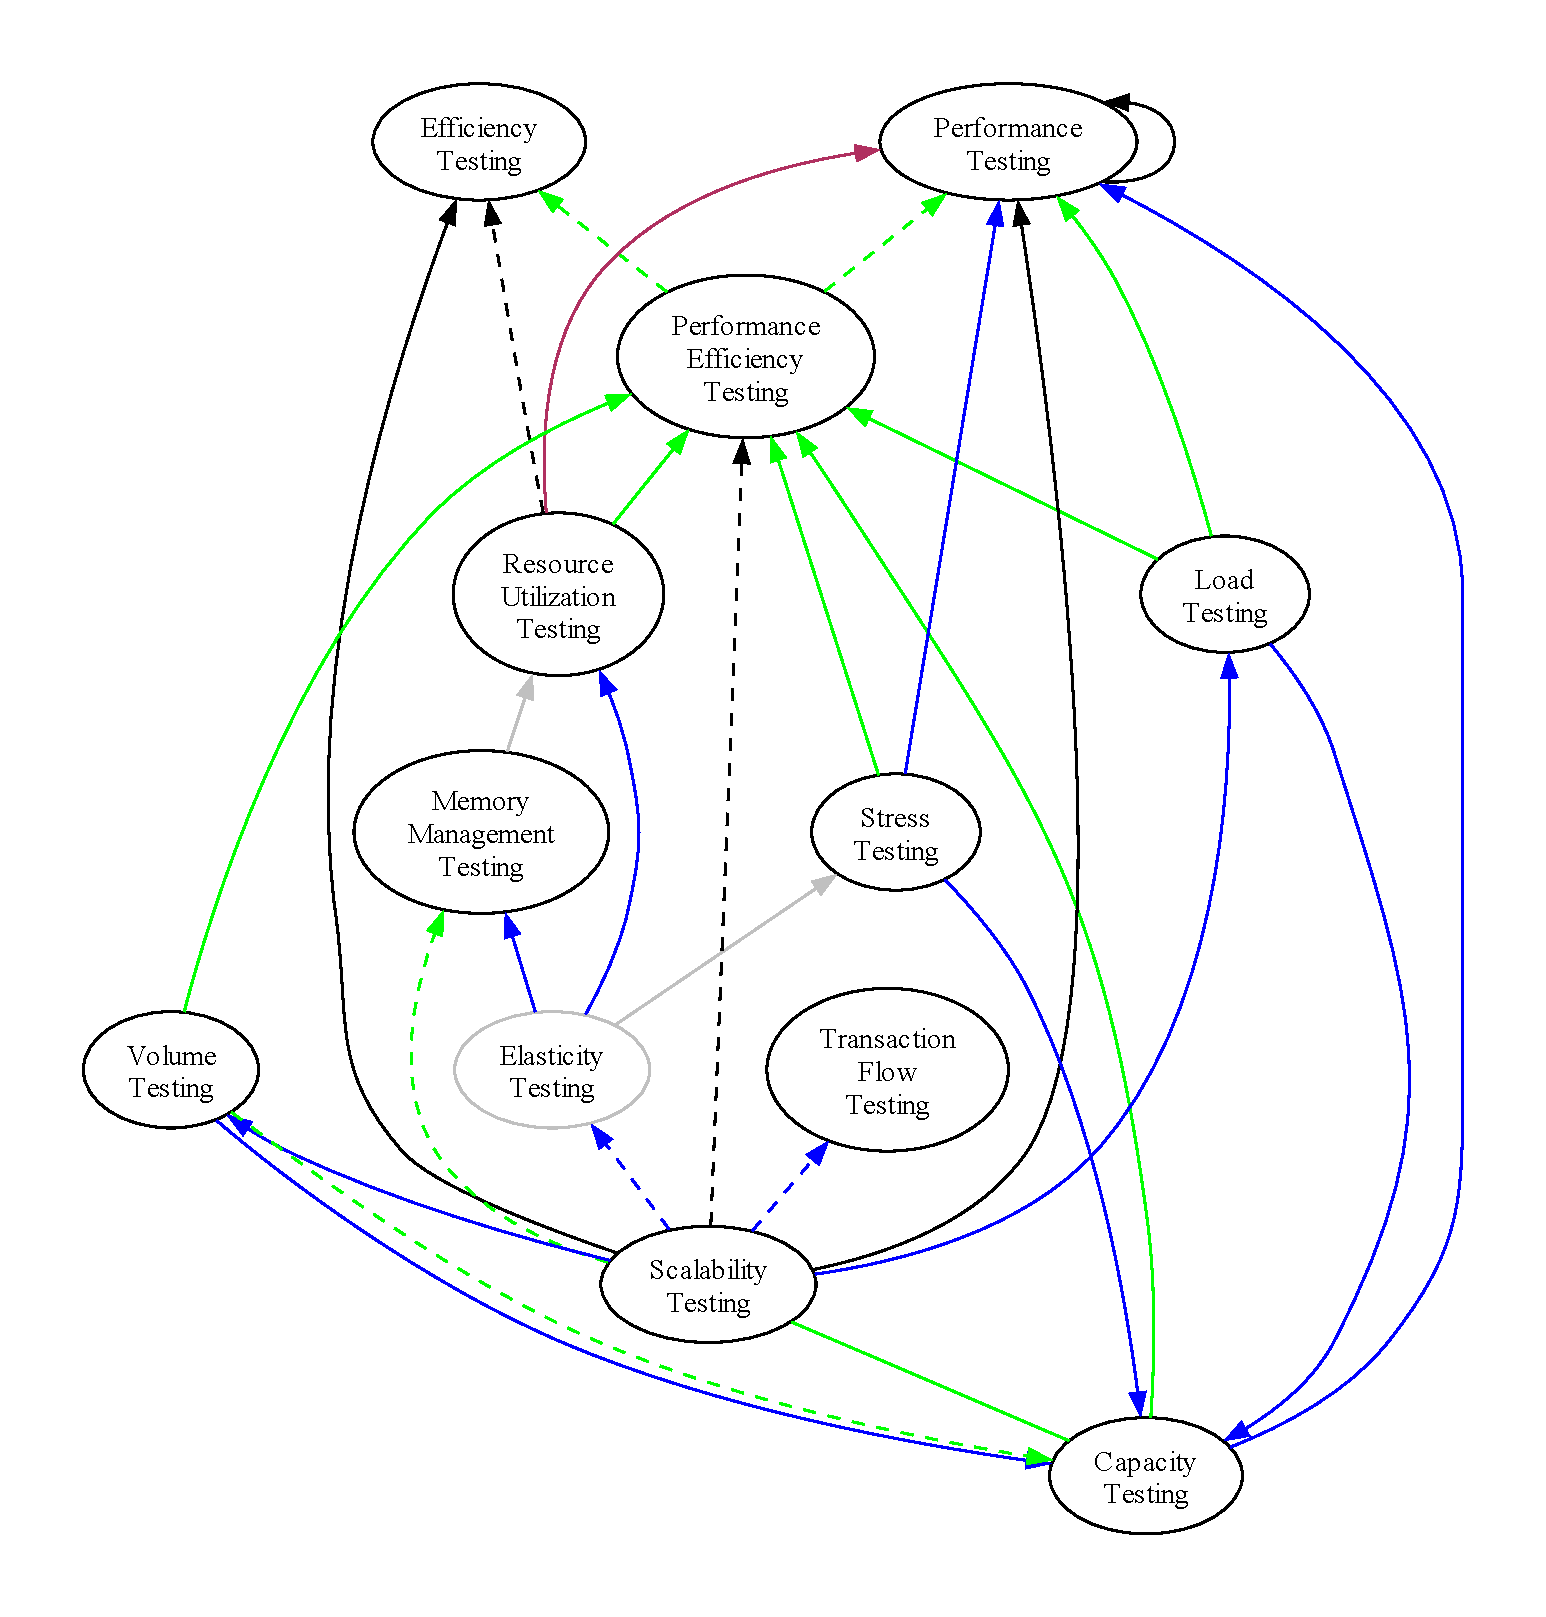
\includegraphics[width=\linewidth]{assets/graphs/scalabilityGraph.pdf}
            \caption{Graph of current relations.}
            \label{fig:scal-graph-current}
        \end{subfigure}
        \begin{subfigure}[b]{.475\linewidth}
            \centering
            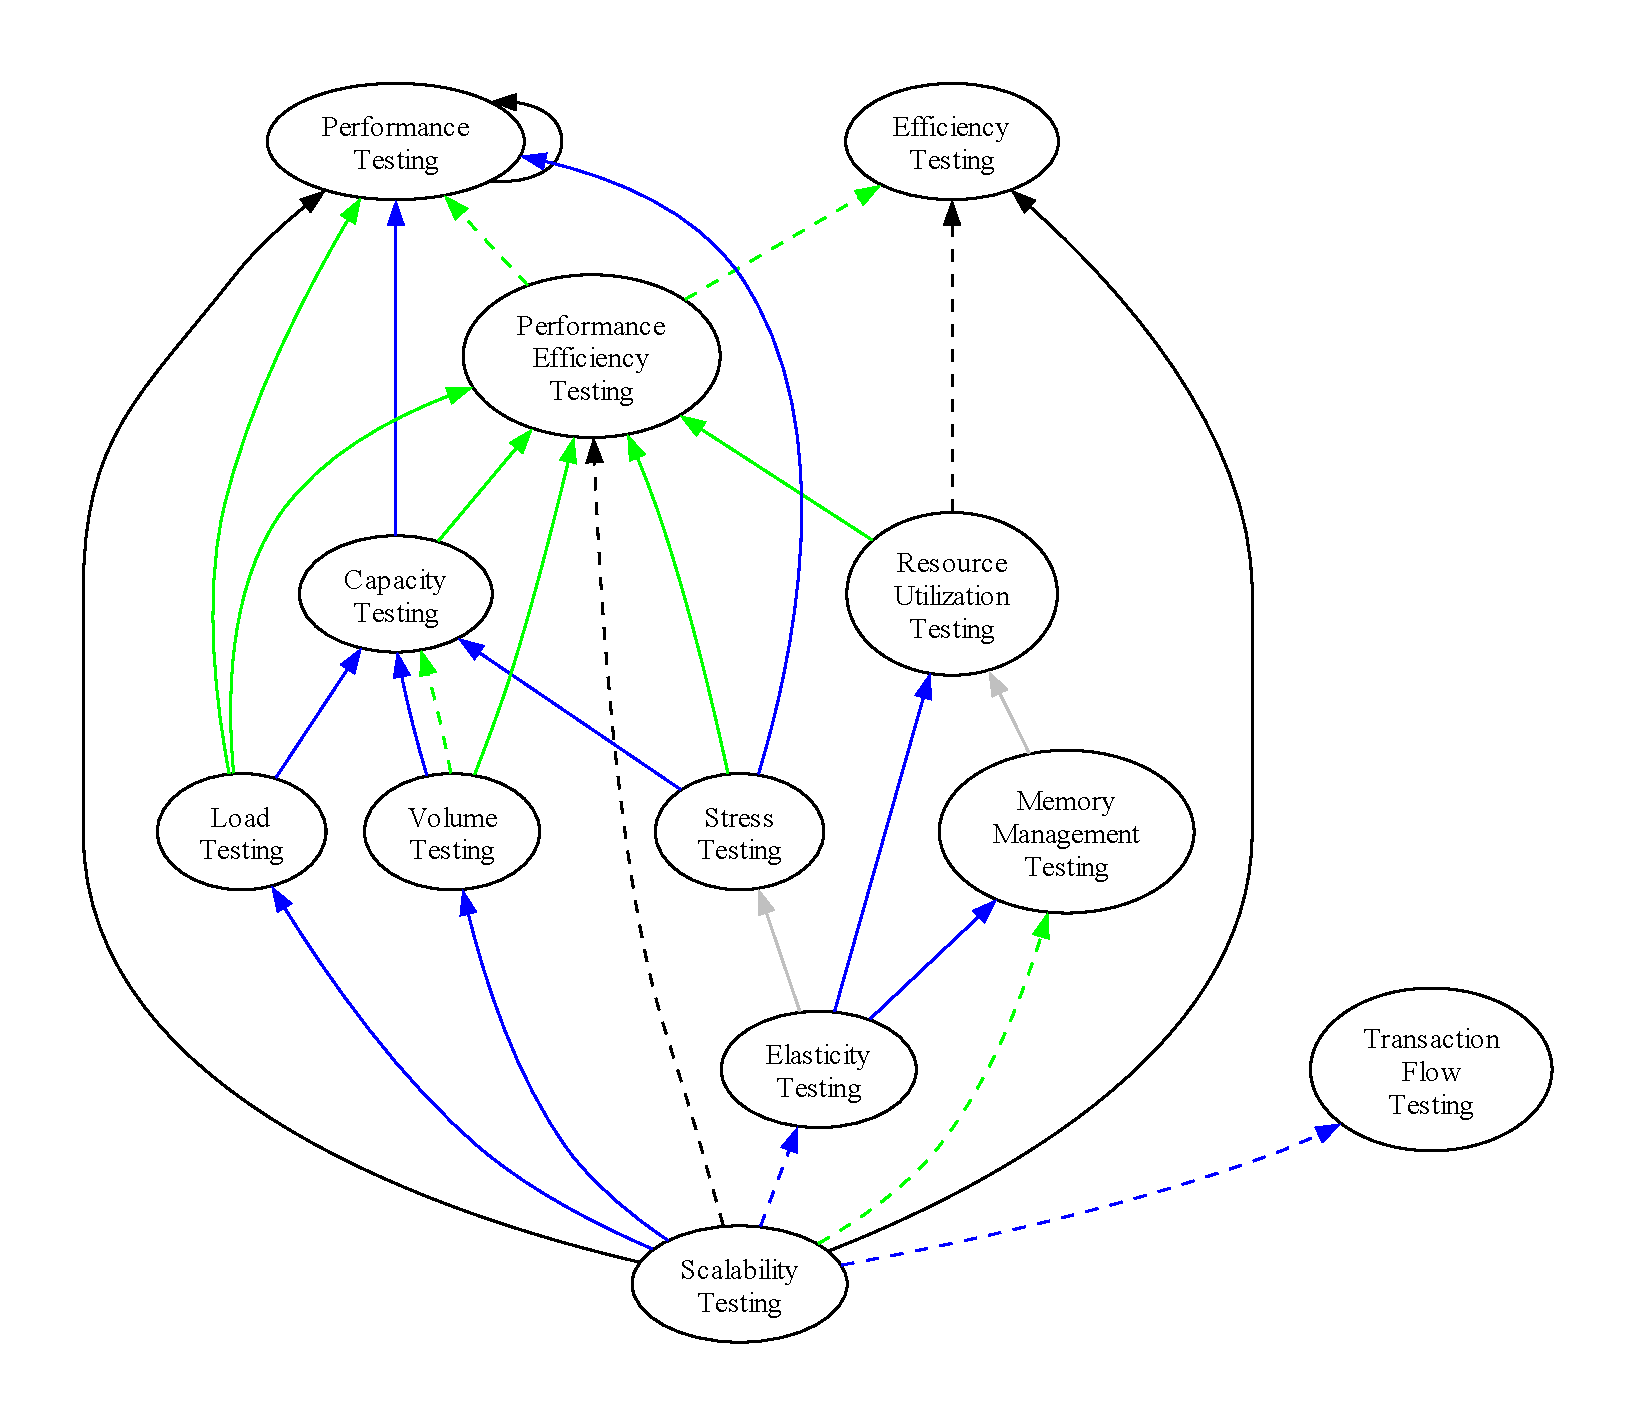
\includegraphics[width=\linewidth]{assets/graphs/scalabilityProposedGraph.pdf}
            \caption{Graph of proposed \ifnotpaper \else \\ \fi relations.}
            \label{fig:scal-graph-proposed}
        \end{subfigure}
        \caption{Graphs of relations between terms related to scalability testing.}
        \label{fig:scalGraphs}
    \end{figure}
}

\newcommand{\performanceGraph}{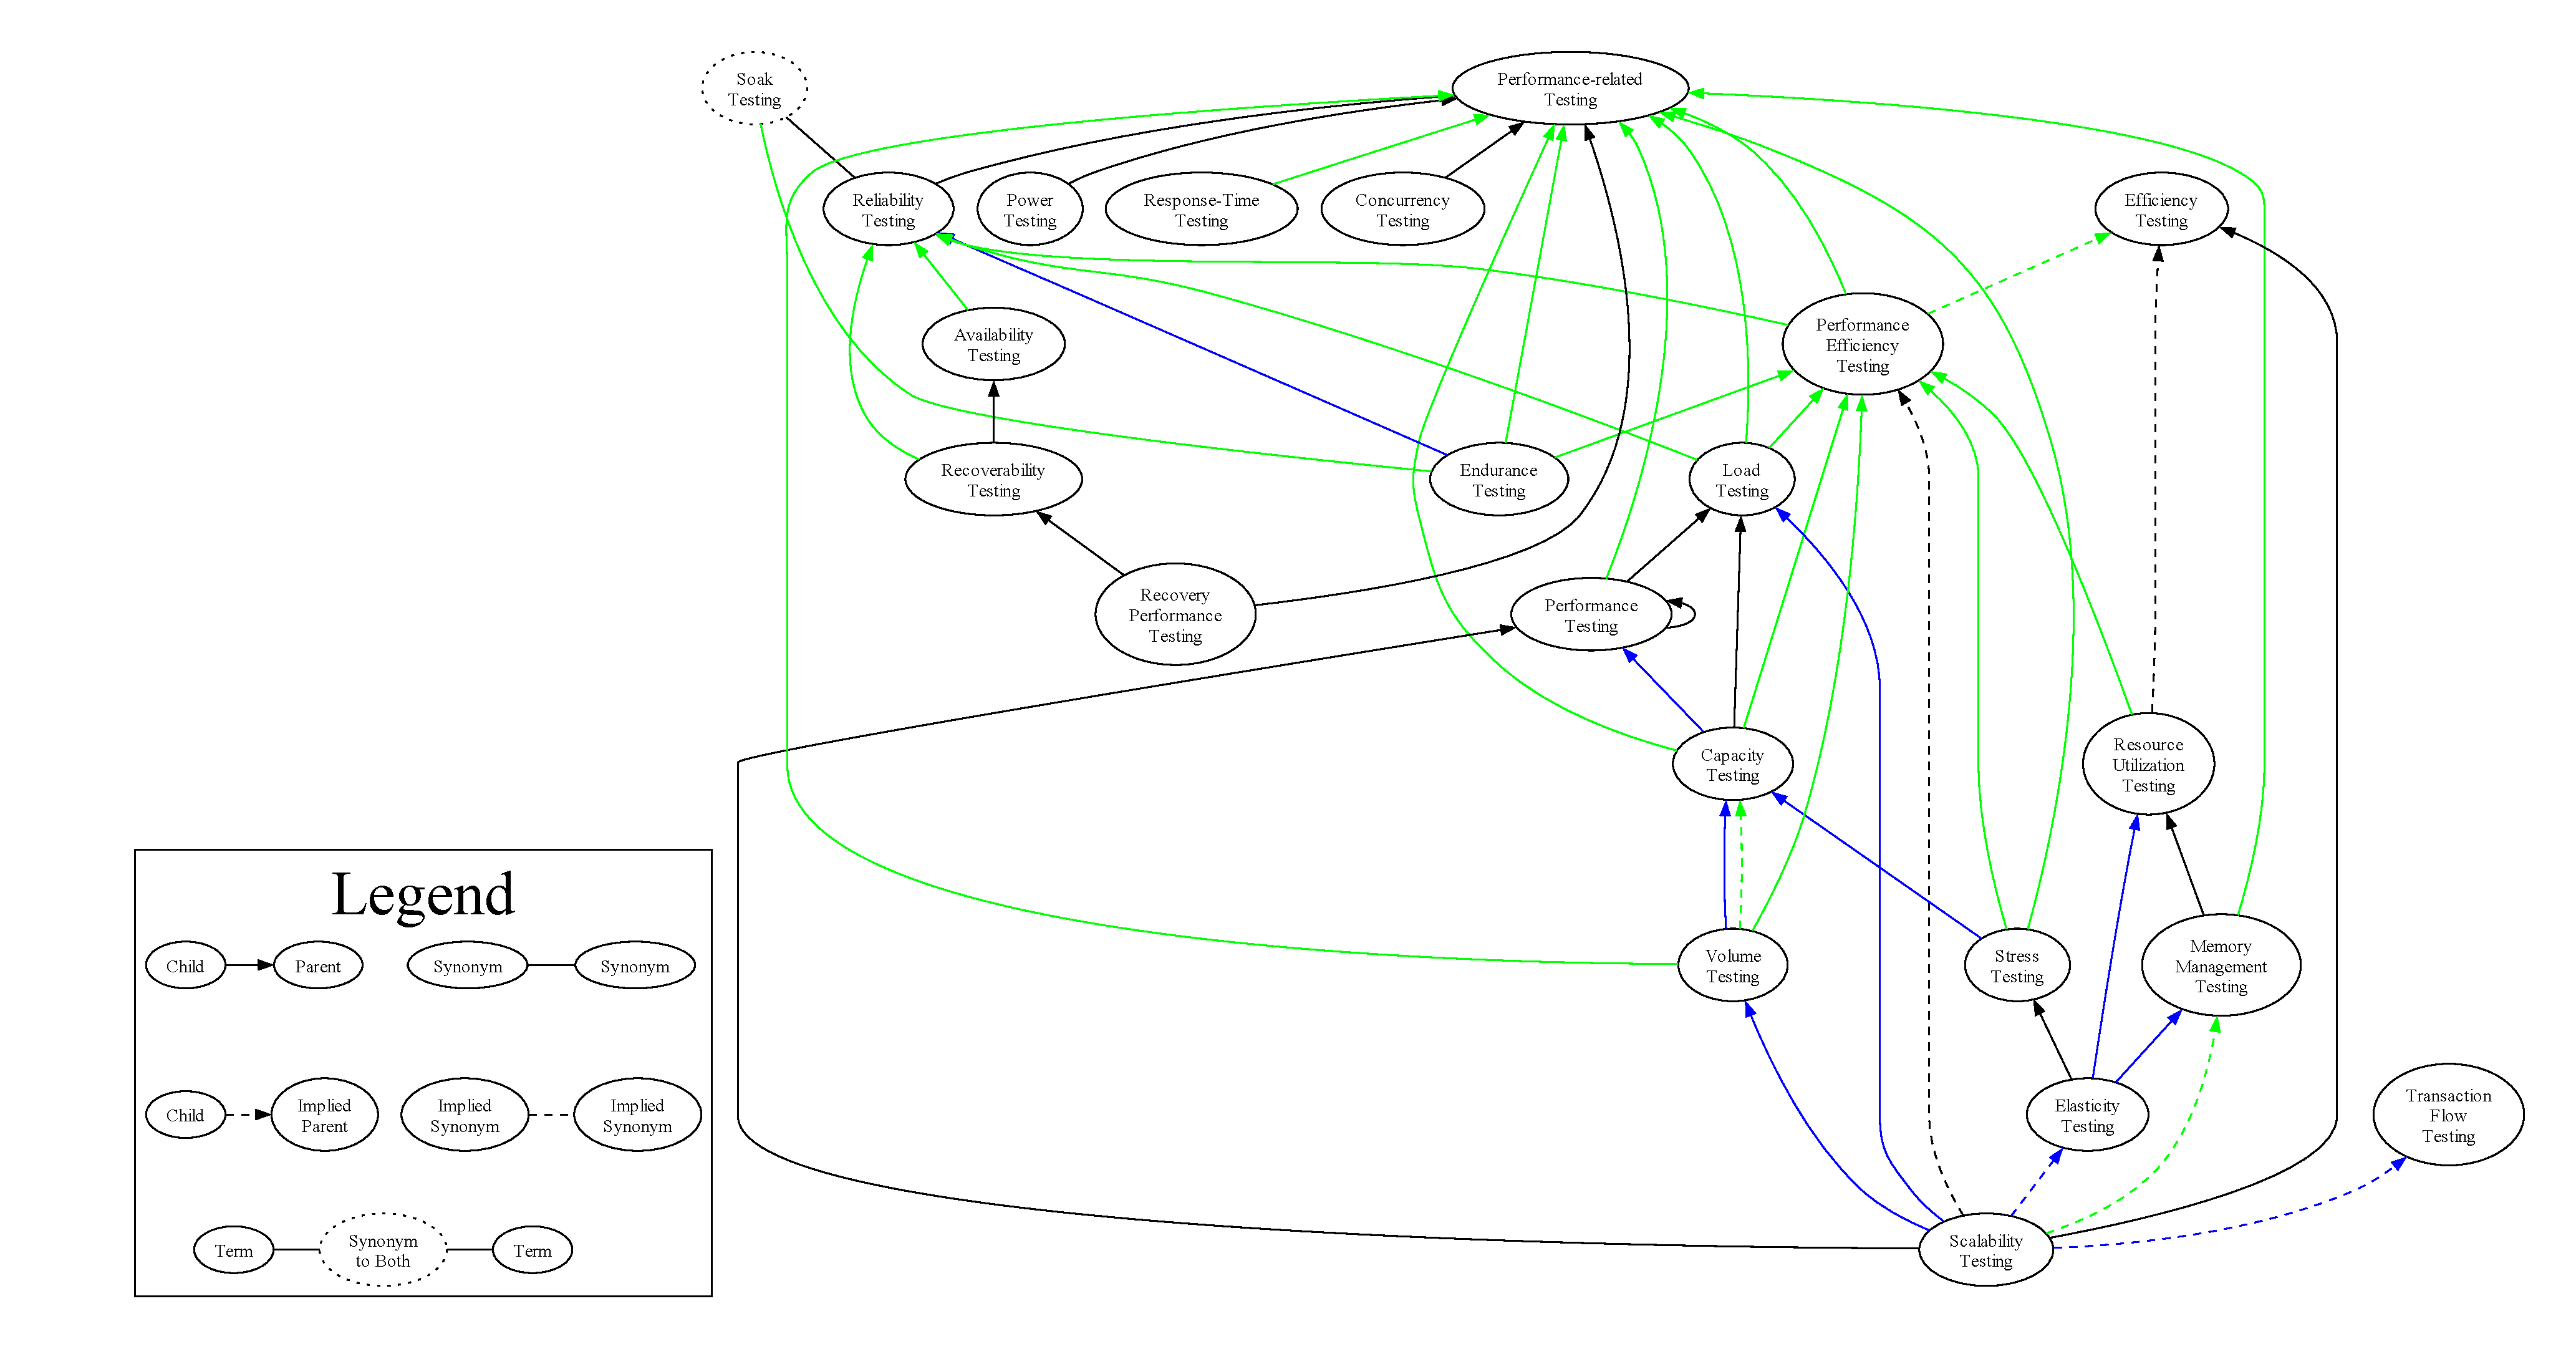
\includegraphics[width=\linewidth]{assets/graphs/performanceProposedGraph.pdf}}

%------------------------------------------------------------------------------
% Images & Figures
%------------------------------------------------------------------------------

\newcommand{\drasilLogo}{assets/images/drasil_logo.png}
\newcommand{\drasilLogoImg}{\begin{figure}[H]
    \centering
    \caption{Drasil's Logo}
    \label{fig:drasilLogo}

    \includegraphics[width=0.6\linewidth]{\drasilLogo}
\end{figure}
}
\newcommand{\refDrasilLogoImg}{\Cref{fig:drasilLogo}}

%------------------------------------------------------------------------------
% Tables
%------------------------------------------------------------------------------

% Organization of files
\newcommand{\organizationTable}{\begin{longtable}[c]{|>{\raggedright}p{0.3\linewidth}|>{\raggedright\arraybackslash}p{0.54\linewidth}|}
    \caption{Template Organization}
    \label{tab:organization}                                              \\

    \hline

    \rowcolor{McMasterMediumGrey}
    \textbf{File/Folder}     & \textbf{Intended Usage \& Description}
    \\ \hline

    \texttt{thesis.tex} & Focal \LaTeX{} file that collects everything and is
    used to build your thesis/report document.
    \\ \hline

    \texttt{Makefile} & A basic \texttt{Makefile} configuration. See
    \texttt{make help} for a list of helpful commands. \\ \hline

    \texttt{build/} & When you build your \acs{pdf}, this folder is used as the
    working directory of LuaLaTeX. Using this allows us to quickly get rid of
    \LaTeX{} build files that can cause problems when we re-build documents. \\
    \hline

    \texttt{manifest.tex} & Basic options that you should certainly configure
    according to your needs.
    \\ \hline

    \texttt{chapters.tex} & All chapters of your thesis should be included here.
    \\ \hline

    \texttt{chapters/} & Enumeration of the chapters of your thesis. I prefer
    using a two-digit indexing pattern for the prefix of file names so that I
    can quickly open up by chapter number using VS Codium. \\ \hline

    \texttt{assets.tex} & Enumeration of the various kinds of ``assets'' in the
    \texttt{assets/} folder. See the file for examples on how you can write your
    extra utility macros. \\ \hline

    \texttt{assets/} & Enumeration of various kinds of ``assets,'' with
    subdirectories for images and figures, tables, and code snippets. \\ \hline

    \texttt{front.tex} & All front matter of your thesis should be included
    here. \\ \hline

    \texttt{front/} & Enumeration of the front chapters of your thesis. These
    chapters should all be numbered using Roman numerals. \\ \hline

    \texttt{back.tex} & All back matter of your thesis should be included here.
    \\ \hline

    \texttt{back/} & Enumeration of the back matter content.
    \\ \hline

    \texttt{acronyms.tex} & List of acronyms you intend to use in your thesis.
    This uses the ``acro'' \LaTeX{} package.
    \\ \hline

    \texttt{macros.tex} & Helpful macros!
    \\ \hline

    \texttt{unicode\_chars.tex} & At times, you might find issues with unicode
    characters, especially in verbatim environments, where you might need to
    manually define them using other font glyphs.
    \\ \hline

    \texttt{mcmaster\_colours.tex} & Macros for the McMaster colour palette.
    \\ \hline

    \texttt{README.md} & Read it!
    \\ \hline

    \texttt{.gitignore} & List of files in the working directory that should be
    ignored by git.
    \\ \hline

    \texttt{latexmkrc} & Used for setting the timezone for latexmk, but can be
    used for other options.
    \\ \hline
\end{longtable}
}

\newcommand{\ieeeCatsTable}{% Conversion to longtblr assisted by GitHub Copilot

\begin{longtblr}[
    note{a} = {Also called ``test phase'' \ifnotpaper (see
            \discrepref{level-phase-syns}) \fi or ``test stage'' \ifnotpaper
            (see \discrepref{stage-level-syns})\else (see relevant synonym
            discrepancies in \Cref{syns})\fi.},
    note{b} = {Also called ``test design technique'' \ifnotpaper
            (\citealp[p.~11]{IEEE2022}; \citealpISTQB{})\else
            \cite[p.~11]{IEEE2022}, \cite{ISTQB}\fi.},
    caption={Categories of testing given by ISO/IEC and IEEE.},
    label={tab:ieeeCats}
    ]{
    colspec={|X[0.09,c,m]X[0.56,m]X[0.3,m]|},
    width = \linewidth, rowhead = 1, hlines
    }
    \thead{Term}                   & \thead{Definition}                           & \thead{Examples} \\
    Test Approach                  & A ``high-level test implementation choice''
    that includes ``test level, test type, test technique, test practice and
    \dots{} static testing'' \citep[p.~10]{IEEE2022} and is used to ``pick the
    particular test case values''
    \citeyearpar[p.~465]{IEEE2017} & black or white box, minimum and maximum
    boundary value testing \citep[p.~465]{IEEE2017}                                                  \\

    Test Level\TblrNote{a}         & A stage of testing ``typically associated
    with the achievement of particular objectives and used to treat particular
    risks'', each performed in sequence \ifnotpaper (\citealp[p.~12]{IEEE2022};
    \citeyear[p.~6]{IEEE2021}) \else \cite[p.~12]{IEEE2022}, \cite[p.~6]{IEEE2021}
    \fi with their ``own documentation and resources''
    \citeyearpar[p.~469]{IEEE2017} % ; more generally, ``designat[es] \dots\ the
    % coverage and detail'' \citeyearpar[p.~249]{IEEE2017} 
                                   & unit/component testing, integration testing,
    system testing, acceptance testing \ifnotpaper (\citealp[p.~12]{IEEE2022};
    \citeyear[p.~6]{IEEE2021}; \citeyear[p.~467]{IEEE2017}) \else
    \cite[p.~12]{IEEE2022}, \cite[p.~467]{IEEE2017}, \cite[p.~6]{IEEE2021} \fi                       \\
    Test Practice                  & A ``conceptual framework that can be
    applied to \dots{} [a] test process to facilitate testing'' \ifnotpaper
    (\citealp[p.~14]{IEEE2022}; \citeyear[p.~471]{IEEE2017}; OG IEEE 2013)
    \else \cite[p.~14]{IEEE2022}, \cite[p.~471]{IEEE2017}
    \fi % ; more generally, a ``specific type of activity that contributes to
    % the execution of a process'' \citeyearpar[p.~331]{IEEE2017} 
                                   & scripted testing, exploratory testing,
    automated testing \citep[p.~20]{IEEE2022}                                                        \\
    Test Technique\TblrNote{b}     & A ``procedure used to create or select a
    test model, identify test coverage items, and derive corresponding test
    cases'' \ifnotpaper (\citeyear[p.~11]{IEEE2022}; similar in
    \citeyear[p.~467]{IEEE2017}) \else \cite[p.~11]{IEEE2022} (similar in
    \cite[p.~467]{IEEE2017}) \fi that ``generate evidence that test item
    requirements have been met or that defects are present in a test item''
    \citeyearpar[p.~vii]{IEEE2021} % ; ``a variety \dots\ is typically
    % required to suitably cover any system'' \citeyearpar[p.~33]{IEEE2022} and
    % is ``often selected based on team skills and familiarity, on the format
    % of the test basis'', and on expectations \citeyearpar[p.~23]{IEEE2022}
                                   & equivalence partitioning,
    boundary value analysis, branch testing \citep[p.~11]{IEEE2022}                                  \\
    Test Type                      & ``Testing that is focused on specific
    quality characteristics'' \ifnotpaper (\citealp[p.~15]{IEEE2022};
    \citeyear[p.~7]{IEEE2021}; \citeyear[p.~473]{IEEE2017}; OG IEEE 2013)
    \else \cite[p.~15]{IEEE2022}, \cite[p.~473]{IEEE2017}, \cite[p.~7]{IEEE2021}
    \fi                            & security testing, usability testing,
    performance testing \ifnotpaper (\citealp[p.~15]{IEEE2022};
    \citeyear[p.~473]{IEEE2017}) \else\cite[p.~15]{IEEE2022},
    \cite[p.~473]{IEEE2017} \fi                                                                      \\
\end{longtblr}
}
\newcommand{\otherCatsTable}{% Defined here so VS Code doesn't freak out
\def\ieeeEquiv{\makecell{IEEE\\Equivalent}}
\def\swebokLevel{{Level\\(objective-\\based)\TblrNote{a}}}

\begin{longtblr}[
    note{a} = {See \flawref{stage-level-syns}.},
    note{b} = {Testing methods and guidances are omitted from this table
            since \citet{BarbosaEtAl2006} do not define or give examples of them.},
    note{c} = {Synonyms for these examples are used by
            \citet[p.~3; OG Mathur, 2012]{SouzaEtAl2017} and
            \citet[p.~3]{BarbosaEtAl2006}.},
    caption={Categories of testing given by other sources.},
    label={tab:otherCats}
    ]{
    colspec={|X[0.08,c,m]|X[0.43,m]|X[0.34,m]|Q[c,m]|},
    width = \linewidth, rowhead = 1
    }
    \hline
    \thead{Term}                           & \thead{Definition}           & \thead{Examples} & \thead{\ieeeEquiv{}} \\
    \hline
    % Guidance                               & none given
    % \citep[p.~3]{BarbosaEtAl2006}          & none given         & Technique?                              \\
    \swebokLevel{}                         & Test levels based on the
    purpose of testing \citep[p.~5\=/6]{SWEBOK2024} that ``determine
    how the test suite is identified \dots\ regarding its consistency
    \dots\ and its composition''
    \citetext{p.~5\=/2}                    & conformance testing,
    installation testing, regression testing, performance testing,
    security testing % reliability testing,
    \citep[pp.~5\=/7 to 5\=/9]{SWEBOK2024} & Type?                                                                  \\
    % Method                                 & none given
    % \citep[p.~3]{BarbosaEtAl2006}          & none given         & Practice?                               \\
    Phase                                  & none given
    %(\citealp[p.~221]{Perry2006}; \citealp[p.~3]{BarbosaEtAl2006})  
                                           & unit testing,
    integration testing, system testing, regression testing (\citealp[p.~221]{Perry2006};
    \citealp[p.~3]{BarbosaEtAl2006})       & Level                                                                  \\
    Procedure                              & The basis for how
    testing is performed that guides the process; ``categorized in[to] testing methods,
    testing guidances\TblrNote{b} and testing techniques''
    \citep[p.~3]{BarbosaEtAl2006}          & none given
    generally; see ``Technique''           & Approach                                                               \\
    Process                                & ``A sequence of
    testing steps'' \citep[p.~2]{BarbosaEtAl2006} ``based on a development technology and \dots\
    paradigm, as well as on a testing procedure''
    \citetext{p.~3}                        & none given                   & Practice                                \\
    Stage                                  & An
    alternative to the ``traditional \dots\ test stages'' %\footnote{See ``Level'' in \Cref{tab:ieeeCats}.}
    based on ``clear technical groupings''
    \citep[p.~13]{Gerrard2000a}            & desktop development testing,
    infrastructure testing,
    % system testing, large scale integration, and
    post-deployment monitoring
    \citep[p.~13]{Gerrard2000a}            & Level                                                                  \\
    Technique                              & ``Systematic
    procedures and approaches for generating or selecting the most suitable test suites''
    \citep[p.~5\=/10]{SWEBOK2024}          & specification-based testing,
    % ``on a sound theoretical basis'' \citep[p.~3]{BarbosaEtAl2006}
    structure-based testing, fault-based testing\TblrNote{c}
    % , experience-based testing, usage-based testing
    (\citealp[pp.~5\=/10, 5\=/13 to 5\=/15]{SWEBOK2024})
    % black-box, white-box, defect/fault-based, model-based testing
    % \citetext{\citealp[p.~3]{SouzaEtAl2017}; OG Mathur, 2012};
    % functional, structural, error-based, state-based testing \citep[p.~3]{BarbosaEtAl2006}
                                           & Technique                                                              \\
    \hline
\end{longtblr}
}
\newcommand{\otherCategorizationsTable}{\def\selecExs{Deterministic Testing\\ Random Testing}
\def\covExs{Input Space Partitioning\\ Graph Coverage\\ Logic Coverage\\ Syntax-based Testing}
\def\execExs{Static Testing\\ Dynamic Testing}
\def\goalExs{Verification Testing\\ Validation Testing}
\def\propExs{Functional Testing\\ Non-functional Testing}

\begin{paperTable}
    \centering
    \begin{minipage}{\linewidth}
        \begin{longtblr}[
            note{\textrm{a}} = {We also consider this categorization meaningful (see \Cref{static-test}).},
            note{\textrm{b}} = {Functional testing is categorized ambiguously (see \Cref{func-test-discrep}) and non-functional testing is uncategorized.},
            caption = {Alternate categorizations given by the literature.},
            label = {tab:otherCategorizations}
            ]{
            colspec = {|X[0.35,c,m]X[0.2,c,m]X[0.35,c,m]|}, width = \linewidth,
            rowhead = 1
            }
            \hline
            \thead{Test Basis}                                        & \thead{Example Approaches} & \thead{Subset of}                                                                                                                      \\
            \hline
            Selection Process \citep[p.~5-16]{SWEBOK2024}             & \selecExs{}                & Technique \citep[pp.~5-12, 5-16]{SWEBOK2024}                                                                                           \\
            \hline
            Coverage Criteria \citep[pp.~18--19]{AmmannAndOffutt2017} & \covExs{}                  & Technique (\citealp[p.~22]{IEEE2022}; \citeyear[Fig.~2]{IEEE2021}; \citealp[p.~5-11]{SWEBOK2024}; \citealp[pp.~47--48]{Firesmith2015}) \\
            \hline
            Execution of Code{\MidTblrNote{\textrm{a}}} (\citealp[p.~214]{KuļešovsEtAl2013}; \citealp[p.~12]{Gerrard2000a};
            \citealp[p.~53]{Patton2006})                              & \execExs{}                 & Approach                                                                                                                               \\
            \hline
            Goal of Testing (\citealp[p.~214]{KuļešovsEtAl2013};
            \citealp[pp.~69--70]{Perry2006})                          & \goalExs{}                 & Approach                                                                                                                               \\
            \hline
            Property of Code \citep[p.~213]{KuļešovsEtAl2013}
            or Test Target \citep[pp.~4--5]{Kam2008}                  & \propExs{}                 & Approach\TblrNote{\textrm{b}}                                                                                                          \\
            \hline
        \end{longtblr}
    \end{minipage}
\end{paperTable}
}

\newcommand{\sntxDiscrepsTable}{\begin{paperTable}
    \centering
    \caption{Breakdown of identified \nameref{sntxDiscreps} by \srcCat{}.}
    \label{tab:sntxDiscreps}
    \begin{minipage}{\linewidth}
        \begin{tabular}{|r|*{6}{cc|}c|}
            \hline
                              & \multicolumn{2}{c|}{\thead{\nameref{wrong}}} & \multicolumn{2}{c|}{\thead{\nameref{miss}}} & \multicolumn{2}{c|}{\thead{\nameref{contra}}} & \multicolumn{2}{c|}{\thead{\nameref{ambi}}} & \multicolumn{2}{c|}{\thead{\nameref{over}}} & \multicolumn{2}{c|}{\thead{\reduns{}}} &                                                                                                                                                                                         \\
            \thead{\srcCat{}} & \thead{Exp}                                  & \thead{Imp}                                 & \thead{Exp}                                   & \thead{Imp}                                 & \thead{Exp}                                 & \thead{Imp}                            & \thead{Exp}             & \thead{Imp}             & \thead{Exp}             & \thead{Imp}              & \thead{Exp}              & \thead{Imp}              & \thead{Total}            \\
            \hline
            \stds{}           & \stdSntxDiscBrkdwn{1}                        & \stdSntxDiscBrkdwn{2}                       & \stdSntxDiscBrkdwn{3}                         & \stdSntxDiscBrkdwn{4}                       & \stdSntxDiscBrkdwn{5}                       & \stdSntxDiscBrkdwn{6}                  & \stdSntxDiscBrkdwn{7}   & \stdSntxDiscBrkdwn{8}   & \stdSntxDiscBrkdwn{9}   & \stdSntxDiscBrkdwn{10}   & \stdSntxDiscBrkdwn{11}   & \stdSntxDiscBrkdwn{12}   & \stdSntxDiscBrkdwn{13}   \\
            \metas{}          & \metaSntxDiscBrkdwn{1}                       & \metaSntxDiscBrkdwn{2}                      & \metaSntxDiscBrkdwn{3}                        & \metaSntxDiscBrkdwn{4}                      & \metaSntxDiscBrkdwn{5}                      & \metaSntxDiscBrkdwn{6}                 & \metaSntxDiscBrkdwn{7}  & \metaSntxDiscBrkdwn{8}  & \metaSntxDiscBrkdwn{9}  & \metaSntxDiscBrkdwn{10}  & \metaSntxDiscBrkdwn{11}  & \metaSntxDiscBrkdwn{12}  & \metaSntxDiscBrkdwn{13}  \\
            \texts{}          & \textSntxDiscBrkdwn{1}                       & \textSntxDiscBrkdwn{2}                      & \textSntxDiscBrkdwn{3}                        & \textSntxDiscBrkdwn{4}                      & \textSntxDiscBrkdwn{5}                      & \textSntxDiscBrkdwn{6}                 & \textSntxDiscBrkdwn{7}  & \textSntxDiscBrkdwn{8}  & \textSntxDiscBrkdwn{9}  & \textSntxDiscBrkdwn{10}  & \textSntxDiscBrkdwn{11}  & \textSntxDiscBrkdwn{12}  & \textSntxDiscBrkdwn{13}  \\
            \papersTbl{}      & \paperSntxDiscBrkdwn{1}                      & \paperSntxDiscBrkdwn{2}                     & \paperSntxDiscBrkdwn{3}                       & \paperSntxDiscBrkdwn{4}                     & \paperSntxDiscBrkdwn{5}                     & \paperSntxDiscBrkdwn{6}                & \paperSntxDiscBrkdwn{7} & \paperSntxDiscBrkdwn{8} & \paperSntxDiscBrkdwn{9} & \paperSntxDiscBrkdwn{10} & \paperSntxDiscBrkdwn{11} & \paperSntxDiscBrkdwn{12} & \paperSntxDiscBrkdwn{13} \\
            \hline
            Total             & \totalSntxDiscBrkdwn{1}                      & \totalSntxDiscBrkdwn{2}                     & \totalSntxDiscBrkdwn{3}                       & \totalSntxDiscBrkdwn{4}                     & \totalSntxDiscBrkdwn{5}                     & \totalSntxDiscBrkdwn{6}                & \totalSntxDiscBrkdwn{7} & \totalSntxDiscBrkdwn{8} & \totalSntxDiscBrkdwn{9} & \totalSntxDiscBrkdwn{10} & \totalSntxDiscBrkdwn{11} & \totalSntxDiscBrkdwn{12} & \totalSntxDiscBrkdwn{13} \\
            \hline
        \end{tabular}
    \end{minipage}
\end{paperTable}
}
\newcommand{\smntcDiscrepsTable}{\begin{paperTable}
    \centering
    \caption{Breakdown of identified \nameref{smntcDiscreps} by \srcCat{}.}
    \label{tab:smntcDiscreps}
    % \begin{minipage}{\linewidth}
    \begin{tabular}{|r|*{6}{cc|}c|}
        \hline
                          & \multicolumn{2}{c|}{\thead{\cats{}}} & \multicolumn{2}{c|}{\thead{\syns{}}} & \multicolumn{2}{c|}{\thead{\pars{}}} & \multicolumn{2}{c|}{\thead{\defs{}}} & \multicolumn{2}{c|}{\thead{\terms{}}} & \multicolumn{2}{c|}{\thead{\cites{}}} &                                                                                                                                                                                                \\
        % \cline{2-10}
        \thead{\srcCat{}} & \thead{Exp}                          & \thead{Imp}                          & \thead{Exp}                          & \thead{Imp}                          & \thead{Exp}                           & \thead{Imp}                           & \thead{Exp}              & \thead{Imp}              & \thead{Exp}              & \thead{Imp}               & \thead{Exp}               & \thead{Imp}               & \thead{Total}             \\
        \hline
        \stds{}           & \stdSmntcDiscBrkdwn{1}               & \stdSmntcDiscBrkdwn{2}               & \stdSmntcDiscBrkdwn{3}               & \stdSmntcDiscBrkdwn{4}               & \stdSmntcDiscBrkdwn{5}                & \stdSmntcDiscBrkdwn{6}                & \stdSmntcDiscBrkdwn{7}   & \stdSmntcDiscBrkdwn{8}   & \stdSmntcDiscBrkdwn{9}   & \stdSmntcDiscBrkdwn{10}   & \stdSmntcDiscBrkdwn{11}   & \stdSmntcDiscBrkdwn{12}   & \stdSmntcDiscBrkdwn{13}   \\
        \metas{}          & \metaSmntcDiscBrkdwn{1}              & \metaSmntcDiscBrkdwn{2}              & \metaSmntcDiscBrkdwn{3}              & \metaSmntcDiscBrkdwn{4}              & \metaSmntcDiscBrkdwn{5}               & \metaSmntcDiscBrkdwn{6}               & \metaSmntcDiscBrkdwn{7}  & \metaSmntcDiscBrkdwn{8}  & \metaSmntcDiscBrkdwn{9}  & \metaSmntcDiscBrkdwn{10}  & \metaSmntcDiscBrkdwn{11}  & \metaSmntcDiscBrkdwn{12}  & \metaSmntcDiscBrkdwn{13}  \\
        \texts{}          & \textSmntcDiscBrkdwn{1}              & \textSmntcDiscBrkdwn{2}              & \textSmntcDiscBrkdwn{3}              & \textSmntcDiscBrkdwn{4}              & \textSmntcDiscBrkdwn{5}               & \textSmntcDiscBrkdwn{6}               & \textSmntcDiscBrkdwn{7}  & \textSmntcDiscBrkdwn{8}  & \textSmntcDiscBrkdwn{9}  & \textSmntcDiscBrkdwn{10}  & \textSmntcDiscBrkdwn{11}  & \textSmntcDiscBrkdwn{12}  & \textSmntcDiscBrkdwn{13}  \\
        \papersTbl{}      & \paperSmntcDiscBrkdwn{1}             & \paperSmntcDiscBrkdwn{2}             & \paperSmntcDiscBrkdwn{3}             & \paperSmntcDiscBrkdwn{4}             & \paperSmntcDiscBrkdwn{5}              & \paperSmntcDiscBrkdwn{6}              & \paperSmntcDiscBrkdwn{7} & \paperSmntcDiscBrkdwn{8} & \paperSmntcDiscBrkdwn{9} & \paperSmntcDiscBrkdwn{10} & \paperSmntcDiscBrkdwn{11} & \paperSmntcDiscBrkdwn{12} & \paperSmntcDiscBrkdwn{13} \\
        \hline
        Total             & \totalSmntcDiscBrkdwn{1}             & \totalSmntcDiscBrkdwn{2}             & \totalSmntcDiscBrkdwn{3}             & \totalSmntcDiscBrkdwn{4}             & \totalSmntcDiscBrkdwn{5}              & \totalSmntcDiscBrkdwn{6}              & \totalSmntcDiscBrkdwn{7} & \totalSmntcDiscBrkdwn{8} & \totalSmntcDiscBrkdwn{9} & \totalSmntcDiscBrkdwn{10} & \totalSmntcDiscBrkdwn{11} & \totalSmntcDiscBrkdwn{12} & \totalSmntcDiscBrkdwn{13} \\
        \hline
    \end{tabular}
    % \end{minipage}
\end{paperTable}}

\newcommand{\testReqsTable}{% To prevent VSCode from aligning things weirdly
\def\typeHead{Testing\\Approach}

\begin{table}[hbtp!]
    \centering
    \caption{Testing Requirements}
    \label{tab:testReqs}
    \begin{tabularx}{\textwidth}{|p{0.14\textwidth}|X|c|c|}
        \hline
        \rowcolor{McMasterMediumGrey}
        \thead{\typeHead}       & \thead{Requirements}                         & \thead{In Drasil?} & \thead{Addable?} \\
        \hline
        Unit testing            & Code modules and their specifications        & ??                 & ??               \\
        Integration testing     & Code modules and their interfaces            & ??                 & ??               \\
        System testing          & Requirements specification; most of the code
                                & ??                                           & ??                                    \\
        Acceptance testing      & Customer requirements and feedback           & ??                 & ??               \\
        Installation testing    & Algorithm for installation; environments to
        test in; method to check
        successful installation & ??                                           & ??                                    \\
        \hline
    \end{tabularx}
\end{table}}
